\documentclass[runningheads]{llncs}
\usepackage[T1]{fontenc}

\usepackage{algorithmic}
\usepackage{algorithm} 
\usepackage{array}
\usepackage{amsmath}
\usepackage{amsfonts}
\usepackage{amssymb}
\usepackage{amsthm}
\usepackage{caption}
\usepackage{comment} 
\usepackage{epsfig} 
\usepackage{fancyhdr}
\usepackage[T1]{fontenc}
\usepackage{geometry} 
\usepackage{graphicx}
\usepackage[colorlinks]{hyperref} 
\usepackage[latin1]{inputenc}
\usepackage{multicol}
\usepackage{multirow} 
\usepackage{rotating}
\usepackage{setspace}
\usepackage{subcaption}
\usepackage{url}
\usepackage{verbatim}
\usepackage{xcolor}
\usepackage{indentfirst}
\usepackage{hyperref}


\hypersetup{
pdftitle={Diabetes prediction using ML},
pdfauthor={Papara Ana Maria},
pdfkeywords={diabetes, ML, feature importance, prediction},
bookmarksnumbered,
pdfstartview={FitH},
urlcolor=black,
colorlinks=true,
linkcolor=black,
citecolor=black,
}


\begin{document}

\title{Optimizing Diabetes Risk Prediction:
Comparative Analysis of Machine Learning Models and
Feature Importance}

\author{Ana-Maria P\u{a}par\u{a} \orcidID{0009-0009-7443-0170}}
\institute{Faculty of Mathematics and Computer Science, Babe\c{s}-Bolyai University \\
\email{ana.maria.papara@gmail.com}\\}

\maketitle
\begin{abstract}
Diabetes is known to be one of the most common diseases in the world today. A significant alternative to traditional diagnostic methods that can be time and resource-consuming is an ML-based approach. With the use of historical health lifestyle and diagnostic data, artificial intelligence can predict someone's risk of developing diabetes. 
This study aims to explore the potential of ML models for the prediction of diabetes based on different health and lifestyle factors. Furthermore, using a feature importance analysis, the objective is to determine the factors that affect the most diabetes condition. By evaluating multiple methods, configurations and datasets, current study aims to identify the most effective approach for predicting diabetes risk.  
For training and prediction, the following 4 models were utilized: Random Forest Classifier (RFC), LightGBM, Decision Tree (DTC) and Naive Bayes. The performance of the models was evaluated on the basis of accuracy, precision, recall and F1-score. The study involved testing these models on two datasets: a smaller one that contains medical attributes (PIMA dataset) and another much larger that incorporates mostly lifestyle factors (derived from the Behavioral Risk Factor Surveillance System Survey from 2022).        The results show that the LightGBM and Random Forest models outperform the other evaluated classifiers. LightGBM achieved the highest accuracy of 86\% in the larger dataset, highlighting the effectiveness of incorporating lifestyle factors. Furthermore, feature importance analysis revealed key predictors, such as weight, height and mobility difficulties to be those that impact diabetes diagnostic the most.       
\keywords{Diabetes \and ML \and Feature importance \and Prediction.}
\end{abstract}


\section{Introduction}
\label{section:introduction}

Diabetes is a chronic health condition that affects millions of people around the world, often leading to severe complications if not diagnosed or poorly managed. Early detection is crucial for effective treatment and better patient outcomes. Traditional diagnostic methods are based on laboratory tests, which can be time-consuming and resource-intensive. Using Artificial Intelligence (AI), this study aims to develop an intelligent system that can predict the onset of diabetes using readily available clinical measurements, thus helping healthcare providers in early diagnosis and intervention. 

The core problem addressed in this study is early and accurate prediction of diabetes using available patient diagnostic data, a task that is often challenging due to the complex nature of diabetes risk factors and their interactions. Detecting diabetes risk early can enable timely intervention and help prevent or mitigate these health problems, improving patient outcomes and reducing healthcare costs.
By training a Machine Learning (ML) model on historical patient data, the algorithm can learn the characteristics of people at risk of diabetes, thereby generating rapid and reliable predictions when provided with new input data. This approach can significantly reduce the need for costly and time-consuming diagnostic procedures, allowing healthcare providers to prioritize high-risk patients for further testing and intervention. 
Formally, the problem can be defined as a binary classification task. 


Most studies addressing diabetes prediction \cite{FEBRIAN202321}, \cite{Dutta}, \cite{GANIE2022100092}, \cite{Xu2024} rely on small datasets, such as PIMA \cite{pimaDataset}, which are limited both in the number of attributes and the number of samples. In addition, these studies often overlook the significance of data augmentation techniques for training datasets and the methods for attribute analysis and selection. Consequently, this research aims to evaluate the performance of ML models trained on larger datasets, to investigate the importance of various attributes and to answer the following research questions:

\textbf{RQ1}: How do different machine learning models (RFC, Gaussian Naive Bayes, DTC, LGBM) compare in terms of accuracy, precision, recall, F1 score and run time for diabetes prediction?

\textbf{RQ2}: What features are the most influential in predicting diabetes according to the Decision Tree Classifier and LightGBM models?

\textbf{RQ3}: How does the performance of machine learning models change when trained on oversampled (using SMOTE and ADASYN) or class-weighted datasets compared to the original?

\textbf{RQ4}: How does the selection of features (all features, SelectKBest and model-based feature importance) impact the performance of machine learning models in the prediction of diabetes?

 The main contribution of the current research is an \textbf{in-depth analysis and comparison} of different models' performances, including detailed evaluation metrics and comparison on different dataset sizes. 
The second contribution is the \textbf{novelty of the dataset}. This study introduces a new data set derived from a large US archive that has not been used before in the prediction of diabetes. Although most of the previous studies have relied on well-known public datasets, the current approach provides novel insights and uncovers new patterns. 
Another original contribution concerns the \textbf{feature importance analysis}. The current study analyzes the importance of the features involved in identifying the key factors that influence diabetes. This contributes to the existing literature by offering new information on diagnostic measurements that can significantly impact the risk of developing diabetes in patients.

This work is organized into five sections as follows: \autoref{section:introduction} provides an overview of the research problem, its significance, the objectives and contributions of this study, \autoref{section:stateOfArt} reviews relevant studies from the literature on diabetes prediction using artificial intelligence and ML models, \autoref{section:proposedApproach} details the proposed approach and the steps followed. Here, the results of the experiments and their interpretation are also depicted.
In the end, \autoref{section:concl} summarizes the important results and conclusions of the article and highlights the strengths and weaknesses of the approach of this study.

\section{Literature review}
\label{section:stateOfArt}

Diabetes prediction through data analysis has gained significant attention due to the increasing potential of ML and AI. 
This section reviews some previous articles that focused on diabetes risk predictions using AI approaches and techniques.

In \cite{FEBRIAN202321}, the Pima Indians Diabetes Database (PIMA)  was used to train the ML model. A detailed description of the PIMA dataset can be found in \autoref{section:dataDescription}.
The main objective of this research was to compare various ML algorithms to see which one suits the best for the prediction of diabetes based on several health attributes. The researchers compared the accuracies of two different ML algorithms: \textbf{K-Nearest Neighbor}, which is based on supervised learning techniques and \textbf{Naive Bayes}, a probabilistic classifier based on the Bayesian theorem. 
Both models were trained on eight health-related attributes to predict the presence of diabetes as a binary outcome. Eight experiments were conducted that differed by the split factor for the test and training data. The percentage of training data ranges from 80 to 10, in each experiment decreasing by 10. 
To evaluate the models, researchers used accuracy, precision and recall and then compared the results for the models. The best results were obtained in the first experiment that had a split of 80-20 for training and test. In this case, the KNN algorithm produced an accuracy of 77.92\%, while Naive Bayes had an accuracy of 78.57\%. Regarding the other experiments, most of the time, the Naive Bayes obtained better results than the KNN, having an average accuracy of 76.07\%, while the KNN only 73.33\%.


The authors of \cite{Dutta} also used the PIMA dataset, but removing patients with missing values. Remaining with only 392 observations, the features in the data set are: number of pregnancies, glucose level, diastolic measure of blood pressure, triceps (value measured in millimeters that estimate body fat), insulin, body mass index, age, history of diabetes in family and a binary variable for diabetes test.
The main goal of the study was to identify the critical health aspects that impact diabetes in a patient. In addition to this, the researchers attempted to improve the accuracy of the prediction by training various ML algorithms and comparing the results.
Three studies with three different algorithms for binary classification have been conducted: Logistic Regression (LogReg), Support Vector Machines (SVM) and Random Forest Classifier (RFC). The data set was divided into train and test in a ratio of 67\% and 33\%. 
Because the data set was imbalanced, the researchers chose to evaluate the models using only F1 and recall metrics. RFC was the most ideal algorithm for predictions with an accuracy of around 79.1\% and having the highest true positive and true negative values. The feature importance analysis performed on RFC highlighted that \textbf{glucose} has the highest importance with 0.21, followed by \textbf{insulin} with 0.19 and \textbf{age} with 0.13 score.

A study \cite{GANIE2022100092} from 2022 uses a private data set collected using offline and online forms between 2019 and 2021 in India. The form was designed with the help of medical field specialists and has been distributed to cover as many areas as possible. The resulting data set consists of 1939 records and 11 features. In addition to the features from PIMA dataset, this one includes more lifestyle parameters such as smoking and drinking habits, along with patient weight, height and variables related to urination (number of times of passing urine in a day/night), thirst (number of times of drinking water in a day/night) and fatigue (if the subject feels fatigued or not). 
This study aimed to develop a model based on ML and ensemble learning techniques to predict diabetes using the collected data.
To enhance the accuracy of the predictions, the researchers combined different ensemble techniques and ML models. Using the Bagging method, they analyzed Bagged Decision Tree (bagged DT), RFC and Extra Tree algorithms. AdaBoost and Stochastic Gradient Boosting have been used through the Boosting method. Then, finally, LogReg, SVM and DTC have been used via Voting method. 
Performance of the models was evaluated using metrics like training accuracy, testing accuracy, miss classification rate and running time. Among all models, the Bagged DT algorithm achieved the highest testing accuracy rate of 99.14\% followed by Stochastic Gradient Boosting with 98.45\% and RFC with 93.64\%. In terms of runtime, the boost models performed the best, both running in 0.03 seconds. A statistical feature importance analysis showed that all features, except \textit{sex} significantly contribute to outcome prediction, with \textbf{urination}, \textbf{weight} and \textbf{thirst} being the most influential. 

Other study \cite{Xu2024} performed in China in 2024 uses a data set from the 2015 Behavioral Risk Factor Surveillance System (BRFSS), which includes 30,691 records and 14 key variables such as age, gender, BMI, high blood pressure, high cholesterol, smoking, stroke, exercise, fruit and vegetable consumption, alcohol use, difficulty walking, education and income. 
The primary goal of this research is to analyze the factors that contribute to diabetes and determine their statistical significance. 
The study employs a Binary LogReg model to evaluate the relationship between the selected variables and the presence of diabetes. This statistical approach allows the identification of significant predictors by examining how each factor influences the likelihood of developing diabetes. 
The author found that the factors that have the most significant impact on diabetes risk are: \textbf{stroke} (74.33\%), \textbf{walk difficulty} (73.64\%) and \textbf{high blood pressure} (67.08\%). In contrast, exercise, fruit consumption, alcohol intake and education are the features with the lowest impact on diagnosis.



\section{Research design and findings}
\label{section:proposedApproach}

\subsection{Overview}

The current study aims to evaluate and compare the performance of multiple ML models, including Random Forest Classifier (RFC), Naive Bayes, Decision Tree Classifier (DTC) and LightGBM (LGBM) \cite{aurelien2019hands}.  
Each model is trained and tested on a structured data set containing diagnostic and lifestyle characteristics, in an attempt to assess its effectiveness in predicting diabetes (following the pipline presented in \autoref{algorithm}). 
To ensure comprehensive performance, the models are evaluated based on the following metrics: \textbf{accuracy} (overall correctness of the predictions), \textbf{ precision} (proportion of correctly predicted positive cases),  \textbf{recall} (model's ability to detect actual positive cases), \textbf{F1} score and   \textbf{run time}.

The first experiment evaluates the following ML models: RFC, Gaussian Naive Bayes, LGBM and DTC on their ability to predict diabetes risk based on the PIMA Indians Diabetes dataset, which consists of 768 records. The objective was to determine the best performing model comparing them using evaluation metrics. 
In the second experiment, a much larger size data set is used to determine if the models maintain their predictive accuracy. The new data set contains over 445,000 records, but it involves a completely different set of attributes compared to PIMA. Dealing now with more complex data, the experiments were structured according to different key dimensions:  \textbf{number of features} (all 15 features, features selected by \textbf{SelectKBest} before model building, features identified based on their importance in the predictive model), 
\textbf{data variations} (original data set, data oversampled using SMOTE, data oversampled using ADASYN), 
\textbf{training approach} (standard training, training with class weights).


Understanding the impact of individual characteristics on model prediction is important for clinical relevance. This study employs a feature importance analysis in two selected models: DTC and LGBM. These models have built-in methods to provide scores for each independent feature based on how much the feature contributes to the target outcome. 
By integrating feature selection with model evaluation, the objective is to determine the optimal combination of ML techniques for an accurate and efficient prediction of the risk of diabetes.


\begin{figure}[htbp]
\centering
    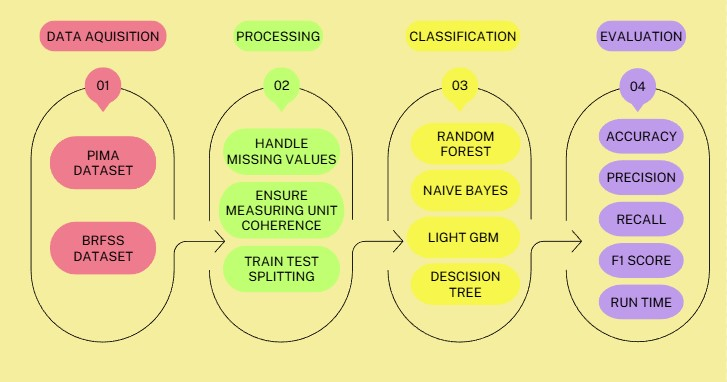
\includegraphics[width=0.5\linewidth]{images/steps.jpg}
    \captionof{figure}{Algorithm steps details}
    \label{algorithm}
\end{figure}


\subsection{Data description}
\label{section:dataDescription}
\subsubsection{PIMA dataset.}

The PIMA Indians Diabetes Dataset \cite{pimaDataset} was collected by the US National Institute of Diabetes and Digestive and Kidney Diseases from a population of 768 women over 21 years of age, of Pima Indian heritage, in the late 1990s. The outcome tested was diabetes, 258 tested positive and 500 negative. Therefore, there is one target variable (dependent) and eight other attributes that describe the health measurements presented in \autoref{tab:comp}. 


\subsubsection{BRFSS dataset.}

This data set was obtained manually by filtering and processing the 2022 BRFSS Survey Data \cite{BRFSS2022}. The \textbf{Behavioral Risk Factor Surveillance System (BRFSS)} is a large-scale ongoing health survey conducted by the Centers for Disease Control and Prevention (CDC) in the United States. Established in 1984, it collects self-reported data on health-related risk behaviors, chronic diseases and preventive health practices from adults through telephone interviews. BRFSS covers topics such as \textbf{smoking}, \textbf{alcohol use}, \textbf{physical activity}, \textbf{diet} or \textbf{chronic conditions}, making it one of the most comprehensive sources of public health data. The data set is widely used for epidemiological research, policymaking and public health interventions. 
To prepare data from the 2022 BRFSS survey for the prediction of diabetes, the data set was first filtered to retain only the most relevant characteristics. The survey results comprise 445,132 records and include 326 variables. Given the large number of variables, a careful selection process was applied to keep the attributes that are the most likely to impact the risk of diabetes. This selection was based on previous research, focusing on factors that may be relevant in the prediction of diabetes. 
Filtering and transformation were performed using Python and the Pandas library. The raw data set, initially in an XPT transport format, was processed into a clean CSV file that contained only the selected attributes. Unnecessary columns were dropped and categorical variables were standardized for consistency. The final version of the data set consists of 444,046 instances (after preprocessing) and 15 attributes that are detailed in \autoref{tab:comp}. 
In addition to the information provided in \autoref{tab:comp}, all categorical variables contain a third value: "7" that encloses "don't know / not sure" and "refuse" answers. 


\begin{table}[ht!] 
    \centering
    \tiny
    \begin{tabular}{|l|c|c|c|c|c|c|c|} 
        \hline
        \multicolumn{3}{|c|}{Reference} & \cite{FEBRIAN202321} & \cite{Dutta} & \cite{GANIE2022100092} & \cite{Xu2024} & new \\ \hline
        \multicolumn{3}{|c|}{Dataset} & PIMA & PIMA & private & BRFSS & BRFSS \\ \hline
        \multicolumn{3}{|c|}{\#samples} & 768 & 392 & 1939 & 30691 & 445132\\ \hline 
        \multicolumn{3}{|c|}{\#features} & 8 & 8 & 10 & 14 & 14\\ \hline
        pregnancies & numeric & $[0, 17]$  & \checkmark & \checkmark & & & \\ \hline
        glucose & numeric & $[0, 199]$  &\checkmark & \checkmark & & & \\ \hline
        blood pressure & numeric & $[0, 122]$ & \checkmark & \checkmark & & & \\ \hline
        skin thickness & numeric & $[0, 99]$ & \checkmark & \checkmark & & & \\ \hline
        insulin & numeric & $[0, 864]$  & \checkmark & \checkmark & & & \\ \hline
        BMI &  numeric & $[0, 67.1]$ & \checkmark & \checkmark & &  \checkmark & \\ \hline
        age & numeric & $[21, 81]$ & \checkmark & \checkmark & \checkmark &  \checkmark & \\ \hline
        history of diabetes & numeric &  $[0.08, 2.42]$ & \checkmark & \checkmark &  \checkmark & & \\ \hline
        gender & categorical & male / female & & & \checkmark & \checkmark & \checkmark\\ \hline

        smoking & categorical & Yes / No & & & \checkmark & \checkmark & \\ \hline
        drinking & categorical & Yes / No & & & \checkmark & \checkmark & \\ \hline
        weight & numeric & $[15, 160]$& & & \checkmark & & \checkmark \\ \hline
        height & numeric & $[60, 250]$ & & & \checkmark & & \checkmark \\ \hline
        urination & numeric & $[2,15]$ & & & \checkmark & & \\ \hline
        thirst & numeric & $[1,15]$ & & & \checkmark & & \\ \hline
        fatigue & categorical & Yes / No & & & \checkmark & & \\ \hline
        high blood pressure & categorical & Yes / No & & & & \checkmark & \\ \hline
        high cholesterol & categorical & Yes / No & & & & \checkmark & \\ \hline
        stroke & categorical & Yes / No & & & & \checkmark & \\ \hline
        exercise & categorical & Yes / No & & & & \checkmark & \\ \hline
        fruit consumption & categorical & Yes / No & & & & \checkmark & \\ \hline
        vegetable consumption & categorical & Yes / No & & & & \checkmark & \\ \hline
        difficulty walking & categorical & Yes / No & & & & \checkmark & \checkmark \\ \hline
        education & categorical & 1/2/3/4/5/6 & & & & \checkmark & \\ \hline
        income & categorical & 1/2/3/4/5/6/7/8  & & & & \checkmark & \\ \hline       
        sleep time & numeric & $[1, 24]$ & & & & & \checkmark\\ \hline
        heart attack ever &categorical & Yes / No & & & & & \checkmark\\ \hline
        heart disease & categorical & Yes / No & & & & & \checkmark\\ \hline
        asthma & categorical & Yes / No & & & & & \checkmark\\ \hline
        any cancer & categorical & Yes / No & & & & & \checkmark\\ \hline
        pulmonary disease & categorical & Yes / No & & & & & \checkmark\\ \hline
        depressive disorder & categorical & Yes / No & & & & & \checkmark\\ \hline
        kidney disease & categorical & Yes / No & & & & & \checkmark\\ \hline
        is deaf & categorical & Yes / No & & & & & \checkmark\\ \hline
        is blind & categorical & Yes / No & & & & & \checkmark\\ \hline
        \multicolumn{3}{|c|}{Data - output} & 0 / 1 & 0 / 1 & 0 / 1 & 0 / 1 & 0 / 1 \\ \hline
        \multicolumn{3}{|c|}{ML performance (KNN)} & 77.92  & & & & \\ \hline
        \multicolumn{3}{|c|}{ML performance (Naive Bayes)} & 78.57  & & & & 85.00  \\ \hline
        \multicolumn{3}{|c|}{ML performance (LogReg)} & & 79.10  & & 72.80  & \\ \hline
        \multicolumn{3}{|c|}{ML performance (SVM)} & & 79.70  & 89.51  & & \\ \hline
        \multicolumn{3}{|c|}{ML performance (RFC)} & & 84.00  & 93.64  &  & 84.00 \\ \hline
        \multicolumn{3}{|c|}{ML performance (Stochastic GB)} & & & 98.45  & & \\ \hline
        \multicolumn{3}{|c|}{ML performance (Bagged DT)} & & & 99.14  & & \\ \hline
        \multicolumn{3}{|c|}{ML performance (DTC)} & & & & & 81.00 \\ \hline
        \multicolumn{3}{|c|}{ML performance (LGBM)} & & & & & 86.50 \\ \hline
        
        \multicolumn{3}{|c|}{Feature importance analysis }& & \checkmark & \checkmark & \checkmark & \checkmark \\ \hline
    \end{tabular}
    \caption{Comparison of datasets and results between literature studies and the current one}
    \label{tab:comp}
\end{table}

The filtering process involves excluding all attributes from the original BRFSS survey data that:
\textbf{cannot have any impact on patient diabetes status} (respondent's residence, source of health insurance, educations, screening history, number of removed teeth), 
\textbf{are limited on a short period of time and so their impact decreases} (physical activity during the past 30 days, alcohol consumption during the past 30 days, confusion or memory loss during the past 12 months), 
\textbf{could have impact on diabetes but have too many missing values} (smoking habits, ever had an H.P.V. vaccination, respondent's race, life satisfaction, stress). 
In the next step, on the just obtained dataset, the following changes were applied: 
(1) missing values for the  categorical variables  were marked as "don't know / not sure" answers, 
(2) missing values for the numerical variables were replaced by the average value of the existing values, 
(3) refused answers were also marked as "don't know / not sure" in order to have fewer labels, 
(4) for the output variable (has diabetes) were stored only two values: \textit{positive} and \textit{negative} as prediabetes, borderline and pregnancy diabetes were treated as no diabetes and the missing values, refused and "don't know" answers were dropped, 
(5) weight values were converted to kilograms and 
(6) height values were converted to centimeters.


\subsection{Numerical experiments}

\subsubsection{Experiment 1 - PIMA dataset}

On the PIMA data set, the models were evaluated based on accuracy, precision, recall, F1 score on the test data. The runtime was also used to compare the models. The runtime is measured in milliseconds and includes only the model training time. 
The evaluation of ML models on the PIMA dataset is presented in \autoref{table:PIMA_results} and reveals that the RFC achieved the highest accuracy (74\%), along with strong precision, recall and F1 scores, making it the best performing model in terms of predictive power. Additionally, it maintained a low run-time of 359 milliseconds (0.4 seconds), balancing both efficiency and effectiveness.
LGBM followed closely with an accuracy of 72\%, although it had the longest run time of 515 milliseconds (4.6 seconds), making it computationally more expensive.
The Gaussian Naive Bayes model demonstrated a slightly lower accuracy of 69\%, but performed comparably in precision and had a great run time performing the training in only 15 milliseconds. 
Overall, the RFC stands out as the most effective model for the prediction of diabetes on this data set, although further improvements can be made with parameter tuning and additional data.

\begin{center}
\begin{tabular}{ |c|c|c|c|c|c| } 
 \hline
 Algorithm & Accuracy & Precision & Recall & F1 & train time (ms) \\ 
 \hline\hline
 Random Forest Classifier &  {0.74} & 0.73 & 0.73 & 0.73 & 359 \\ 
 Gaussian Naive Bayes & 0.69 & 0.70 & 0.69 & 0.69 & 15  \\ 
 LightGBM & 0.72 & 0.72 & 0.72 & 0.72 & 515 \\ 
Decision Tree Classifier & 0.66 & 0.65 & 0.66 & 0.65 & 15 \\ 
 \hline
\end{tabular}
\captionof{table}{Model evaluation metrics on PIMA dataset}
\label{table:PIMA_results}
\end{center}

\subsubsection{Experiment 2 - BRFSS dataset.} 

The results obtained on the BRFSS dataset depicted in \autoref{table:allExp}  (column 3) indicate a noticeable improvement in models performance compared to the PIMA dataset, probably due to the larger dataset size and richer feature set. 
LGBM emerged as the best performing model, achieving the highest accuracy of 86\%, making it the most reliable for the identification of diabetes cases. Interestingly, the Categorical Naive Bayes closely followed with an accuracy of 85\%, demonstrating that a probabilistic approach can be highly effective when the dataset contains categorical features. Despite its strong performance, the RFC, which has an accuracy of 84\%, took significantly longer to run, suggesting that while it is a robust model, it may not be the most efficient choice for large-scale applications. 
Unlike in the PIMA dataset experiment, where DTC struggled, here the DTC performed reasonably well with 81\% accuracy, suggesting that the dataset's structure allows for better boundary learning. Another interesting observation is that LGBM, despite its superior performance, ran significantly faster (3.7 seconds) than RFC, highlighting the advantage of gradient boosting techniques in balancing both speed and accuracy. 
The differences in model rankings between the two datasets reinforce the idea that model performance is highly data dependent, highlighting the importance of dataset-specific tuning rather than a one-size-fits-all approach.


\subsubsection{Experiment 3 - Feature importance analysis.}

Feature analysis is an important step in results analysis because it helps determine which variables have the most influence on model predictions. Understanding the impact of each feature allows for easier understanding of the model, improved performance and potential feature selection. In addition, analysis of feature importance has clinical relevance because it helps identify which factors contribute the most to the risk of disease.
In this study, a feature importance analysis was conducted using RFC, LGBM and DTC. 
Because Naive Bayes models simplify the computation and make the algorithm more efficient by assuming feature independence, it is known to be not suitable for feature importance analysis.

\textbf{LGBM} provides importance scores based on how often a feature is used for splitting and how much it improves the ability of the model to predict the correct results. Two primary metrics \cite{lightGBM} are used: \textit{split importance}, which counts the number of times a feature is used as a decision node and \textit{gain importance}, which measures the total gain of information provided by the feature across all splits. In other words, \textit{gain} value measures how much better the split makes predictions compared to before the split, while \textit{split} value measures how frequently the feature was chosen as the splitting criterion. However, a high split count does not necessarily mean that the feature is highly influential; it might just be frequently used. So, gain-based importance is generally more reliable, as it reflects both frequency and impact on model performance. 
On the other hand, the \textbf{DTC} assigns importance scores based on how effectively each feature reduces uncertainty (impurity) in the dataset when making splits. The features that contribute the most to distinguishing between diabetic and non-diabetic individuals receive higher scores, while those with minimal impact are ranked lower. 
Similarly to DTC, the \textbf{RFC} determines the importance of the features by measuring how much each contributes to reducing the impurity in all trees in the ensemble. Since RFC aggregates results from multiple decision trees, its feature importance scores are more stable and reliable than those from a single decision tree.

The feature importance analysis on \textbf{LGBM} presented in \autoref{fig:lightGBM_gain_features} and \autoref{fig:lightGBM_split_features} reveal which features are the most commonly used to divide the data (split values) and also  which features are most valuable to improve the accuracy of the model (gain values).
In terms of gain importance, \textit{any\_walk\_difficulty}, \textit{weight}, \textit{kidney\_disease} and \textit{height} play a key role in improving the model accuracy. This suggests that mobility limitations are strongly correlated with the risk of diabetes. On the other hand, \textit{weight}, \textit{height} and \textit{sleep time} are highlighted as the most frequently used features in the decision-making process, having the highest split importance values. However, \textbf{weight} and \textbf{height} are consistently important in both types of importance, while \textbf{depressive disorder} and \textbf{asthma ever} appear to be less influential in both split and gain importance.

\begin{figure}[htbp]
    \centering
    \begin{subfigure}[t]{0.48\textwidth}
        \centering
        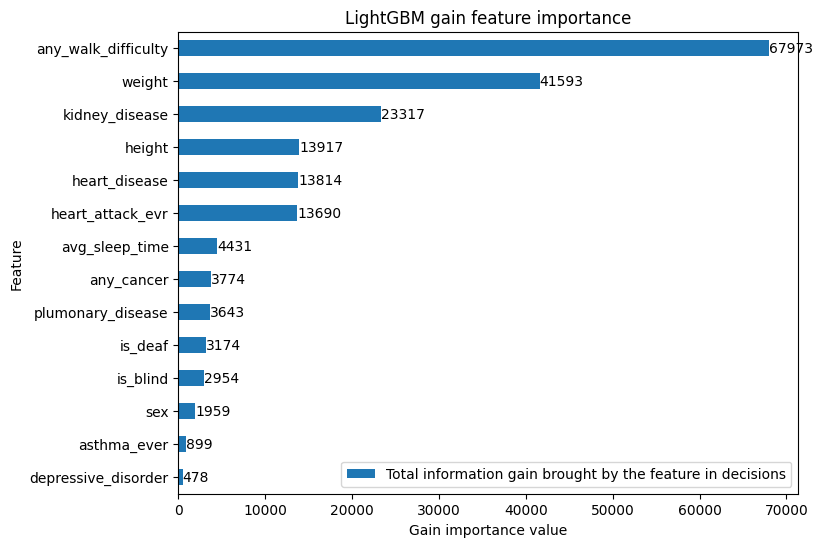
\includegraphics[width=0.99\linewidth]{images/gain_fi.png}
        \caption{LGBM GAIN feature importance}
        \label{fig:lightGBM_gain_features}
    \end{subfigure}%
    ~ 
    \begin{subfigure}[t]{0.48\textwidth}
        \centering
        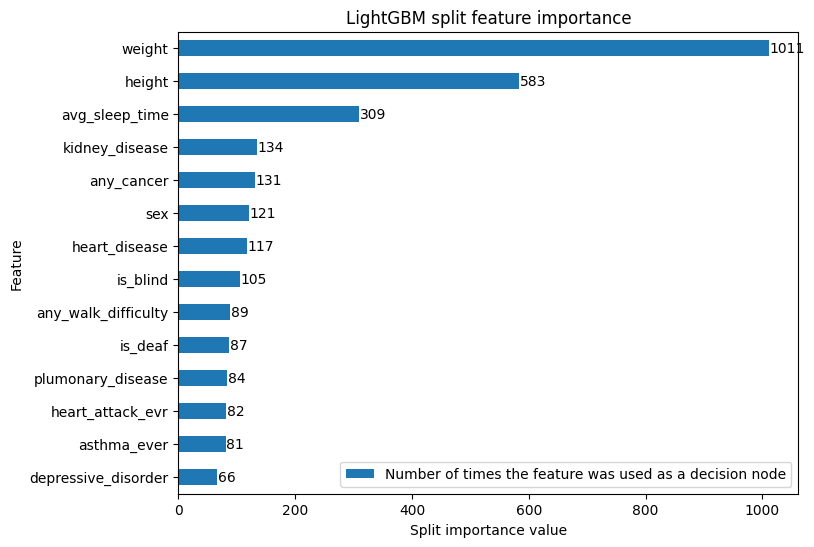
\includegraphics[width=0.99\linewidth]{images/split_fi.png}
        \caption{LGBM SPLIT feature importance}
        \label{fig:lightGBM_split_features}
    \end{subfigure}
    \caption{Feature importance - GAIN and SPLIT}
\end{figure}

On the other hand, the \textbf{DTC} produced a different ranking of important features, exposed in \autoref{fig:DT_feature}. The most influential attributes according to this model were \textit{weight}, \textit{height}, \textit{avg\_sleep\_time}, \textit{any\_walk\_difficulty} and \textit{depressive\_disorder}. Unlike LGBM, which emphasized chronic conditions, DTC placed greater importance on average sleep time and depressive disorder, indicating that lifestyle and mental health factors had a stronger influence on the model output. Weight and height remained among the top features in both models, confirming their relevance in the assessment of diabetes risk. 
   
Feature importance scores from \textbf{RFC}, highlighted in \autoref{fig:rf_feature}, are very similar to the DTC scores, at least in terms of the first part of the ranking. Although the first 4 most influential features remain the same in these 2 models, it can be observed that they have different scores with \textit{weight} counting more in Random Forest. These similarities are due to the fact that both models use impurity reduction to determine splits, so the most important features according to DTC will also tend to be important in the RFC. It is also worth mentioning that in the RFC feature ranking, the \textit{kidney\_disease} takes a higher place, defending \textit{depressive\_disorder}, a fact that is also met in LGBM ranking.

\begin{figure}[htbp]
    \centering
    \begin{subfigure}[t]{0.48\textwidth}
        \centering
        \includegraphics[width=0.99\linewidth]{images/DT_fi.png}
        \caption{DTC feature importance}
        \label{fig:DT_feature}
    \end{subfigure}%
    ~ 
    \begin{subfigure}[t]{0.48\textwidth}
        \centering
        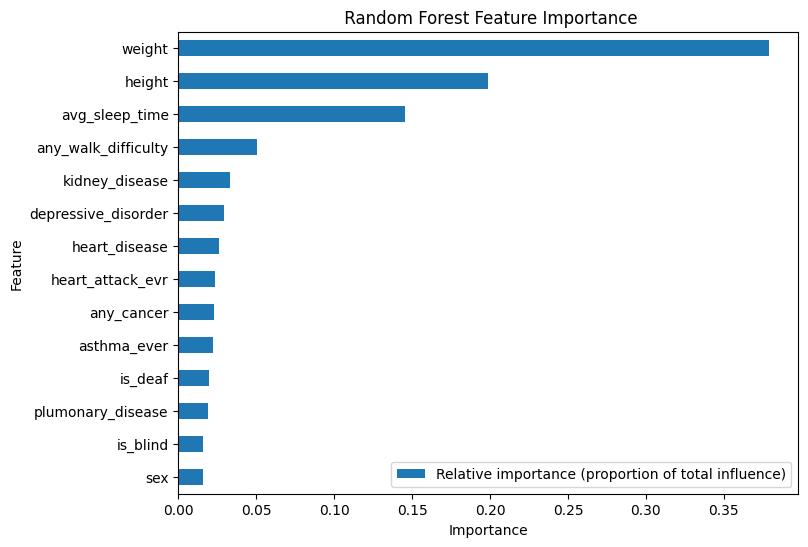
\includegraphics[width=0.99\linewidth]{images/rf_fi.png}
        \caption{RFC feature importance}
        \label{fig:rf_feature}
    \end{subfigure}
    \caption{Feature importance}
\end{figure}

The key differences between the four different approaches for feature importance analysis are the way each model learns and evaluates the contributions of the feature. LGBM, as a boosting algorithm, builds multiple weak learners sequentially, refining feature importance by prioritizing those that consistently reduce error across iterations. In contrast, DTC and RFC rely on building individual trees or ensembles of trees, where feature importance is based on how often features are used in the reduction of impurity. 
The differences in value ranges are because in RFC and DTC (both imported from scikit-learn library) the importance values are, by default, normalized so that they all sum to one.
Regarding the results, it can be observed that features like \textbf{weight} and \textbf{height} are consistently ranked as the most important in all models, indicating their strong influence on the prediction of diabetes.
There is a strong correlation between split importance from LGBM, DTC and RFC feature importance. All three approaches are rating \textit{weight}, \textit{height} and \textit{sleep time} as the features with the highest impact on the output variable. However, it is interesting to see how \textit{depressive disorder} is placed in the top 6 in both DTC and RFC and, at the same time, has the lowest value in the split importance of LGBM.

The findings of this feature importance analysis can be compared with those of similar studies in the literature. 
The study \cite{Xu2024} uses a dataset derived from the 2015 BRFSS survey, but there are notable differences in the feature filtering process compared to the current study. These differences arise due to variations in data filtering, leading to different sets of features being used in each study. As shown in \autoref{ tab:comp} the only common features of both datasets are \textit{gender} and \textit{difficulty walking}. In study \cite{Xu2024} \textit{walking difficulty}  was identified as the second most important feature, followed by \textit{stroke}. In contrast, in the current study, LGBM gain-based feature importance (\autoref{fig:lightGBM_gain_features}) ranked \textit{walking difficulty} as the most influential factor. 

Another relevant study \cite{GANIE2022100092}, although based on a different dataset, includes three common features with the current research: \textit{gender}, \textit{weight} and \textit{height} (as can be observed in \autoref{tab:comp}). 
In that study, weight was assigned an importance of 23\%, being the second most important feature after urination. Height had a minimal influence of 0.03\% and gender was found to be completely insignificant (0\% importance). 
In comparison, if the LGBM gain-based feature importance values (\autoref{fig:lightGBM_gain_features}) were normalized to sum 1,  weight would be similarly influential at 21.26\%, while height played a much larger role at 7.11\%. Additionally, while gender was still relatively irrelevant in both studies, it held slightly higher weight in the current analysis (1.00\%). These variations suggest that although some feature rankings remain consistent across studies, differences in dataset composition, feature engineering and model selection can significantly affect the perceived importance of individual variables.

\subsubsection{Experiment 4 - Class weights} 

One of the challenges in training ML models on the BRFSS dataset is the imbalance between the two classes. Out of 444.045 total respondents, only 61.158 have diabetes, while the remaining 382.887 do not. This imbalance can lead to biased models that favor the majority class, reducing the model's ability to predict diabetes. To avoid this problem, the \textbf{class weighting} was applied. Class weighting is a technique that adjusts the model's learning process by assigning higher importance to underrepresented classes.
\cite{classWeights2023}. 

This ensures that the contribution of each class is balanced in the model learning process. The adjusted weights penalize misclassifications of the minority class more heavily, helping the model pay more attention to the underrepresented class. 
In \autoref{table:allExp} (column 3) are described new computed evaluation metrics for the models that support \textit{class\_weight} parameter. 
After applying class weights to the models that support them (RFC, DTC and LGBM), results showed that this approach did not significantly improve accuracy. RFC maintained nearly the same accuracy of 80\%, while both LGBM and DTC saw a slight decrease in performance. However, an interesting observation is the significant reduction in terms of run-time. The training time was almost halved for LGBM and DTC. This suggests that class weighting may introduce regularization effects, reducing overfitting and allowing models to converge faster.


\subsubsection{Experiment 5 - Resampling}

Considering the fact that applying class weights did not improve the performance of the models, another feasible solution is \textbf{resampling}.
This method involves adjusting the balance between minority and majority classes through up-sampling or down-sampling. In the case of an imbalanced dataset, \textbf{oversampling} involves generating synthetic records for the minority class while \textbf{undersampling} entails removing rows from the majority class. 
Because undersampling can discard valuable data from the majority class, leading to a loss of potentially important information, it is best to choose oversampling. 
\textbf{SMOTE (Synthetic Minority Oversampling Technique)} 
\cite{smote2019}
is a popular oversampling technique that works by identifying the k-nearest neighbors in the feature space for each minority class instance and then creating synthetic examples starting from the original instance and using the difference between the instance and its neighbors. 
\textbf{ADASYN (Adaptive Synthetic Sampling)} 
\cite{adasyn2008}
is an improved version of SMOTE. What it brings over SMOTE is that it adds a random value in the computation process so instead of all the samples being linearly correlated to the parent they have a little more variance. 

In order to ensure a consistent comparison, a single test set was used to evaluate the models trained on different data. Firstly, a subset of 20,000 samples (10,000 positive and 10,000 negative) were held back for testing and the rest of 424,045 were collected in training set. Afterwards, a LGBM model was trained separately on the obtained training set (without any sampling), on the training set oversampled using ADASYN and on the training set oversampled using SMOTE. In the end, the models were evaluated on the balanced test set. The performance of the models was compared both based on confusion matrices (see \autoref{fig:exp2_matrices} ) and based on accuracy, precision, recall and F1 score as shown in \autoref{table:allExp} columns 4 and 5. 


\begin{figure}[htbp]
    \centering
    \begin{subfigure}[t]{0.3\textwidth}
        \centering
        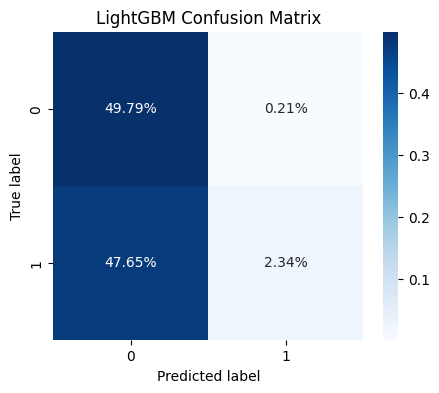
\includegraphics[width=0.99\linewidth]{images/exp2_matrix.png}
        \caption{Original data}
        \label{Fig:exp2_matrix1}
    \end{subfigure}%
    ~ 
    \begin{subfigure}[t]{0.3\textwidth}
        \centering
        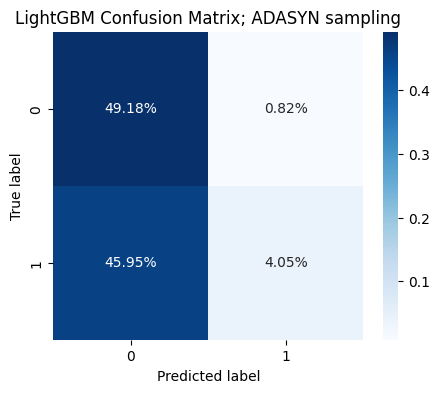
\includegraphics[width=0.99\linewidth]{images/exp2_matrix_adasyn.png}
        \caption{ADASYN data}
        \label{Fig:exp2_matrix_adasyn}
    \end{subfigure}
    ~ 
    \begin{subfigure}[t]{0.3\textwidth}
        \centering
        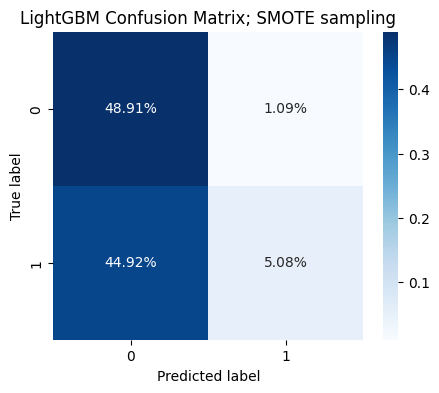
\includegraphics[width=0.99\linewidth]{images/exp2_matrix_smote.png}
        \caption{SMOTE data}
        \label{Fig:exp2_matrix_smote}
    \end{subfigure}
    \caption{Confusion matrices for the LGB models trained on original, ADASYN and SMOTE data; tested on same test set.}
    \label{fig:exp2_matrices}
\end{figure}


It can be observed in the matrices that there is a small improvement from the original model to the models trained on the oversampled data, especially in terms of true positives: increasing from 2.34\% to 4.05\%  in ADASYN and to 5.08\% in SMOTE. Despite this improvement appearance, the measurements presented in \autoref{table:allExp} show a significant decrease in the five evaluation metrics.


\subsubsection{Experiment 6 - Feature selection}

Feature selection can be a crucial step in ML aiming to reduce dimensionality, improve model accuracy and enhance model efficiency \cite{BARBIERI2024123667}. In this study, SelectKBest is used for feature selection along with a manual selection based on feature importance scores computed by DTC. \textbf {SelectKBest} is a univariate feature selection method that selects the top \textbf{k} features based on statistical scoring.  SelectKBest is a filter-based feature selection method; the feature selection process is carried out independently of any specific ML algorithm \cite{selectkbest}. Instead, it relies on statistical measures to score and rank features.
This technique helps to retain only the most relevant features, eliminating those that have a minimal impact on the prediction of diabetes. 


The feature selection process in the current study followed a structured pipeline: 
(1) \textbf{Dataset Preparation}: The data set used was the BRFSS after preprocessing steps. 
(2) \textbf{Feature Selection}: 
(a) SelectKBest was applied to identify the most predictive features based on statistical scores. 
(b) Separately, a DTC was used to calculate the importance of the feature and the first 5 features with the highest importance were selected. 
(3) \textbf{Model Training \& Evaluation}: Three selected feature subsets (first 5 from SelectKBest, first 10 from SelectKBest, first 5 from Decision Tree Classifier) were used to train RFC, LGBM and DTC. Afterwards, the models were evaluated based on accuracy, precision, recall and F1 score. 


SelectKBest was used in two experiments: the first time with the parameter \textit{k=5}, results provided in \autoref{table:allExp} (column 6) and the second time with \textit{k=10}, results provided in \autoref{table:allExp} (column 7).  
Furthermore, an experiment (results in \autoref{table:allExp}, column 8) was conducted using only the subset of the first five features with highest importance computed by the DTC. So, the models were trained again only on the following features: 

\begin{enumerate}
   \item \textbf{Best 5 features computed with \textbf{SelectKBest}}: 
   \textit{any\_walk\_difficulty},
   \textit{is\_blind},
   \textit{is\_deaf},
    \textit{height}, 
   \textit{weight}
      
    \item \textbf{Best 10 features computed with \textbf{SelectKBest}}:    
   \textit{any\_walk\_difficulty},
   \textit{is\_blind},
   \textit{is\_deaf},
    \textit{height}, 
   \textit{weight},
   \textit{kidney\_disease}, 
    \textit{plumonary\_disease}, 
    \textit{any\_cancer}, 
    \textit{asthma\_ever},
    \textit{heart\_attack\_ever}
    
    
     \item \textbf{Best 5 features computed by Decision Tree Classifier}: 
     \textit{weight}, 
     \textit{height}, 
     \textit{avg\_sleep\_time}, \textit{any\_walk\_difficulty}, \textit{depressive\_disorder}
\end{enumerate}

While both feature selection techniques (SelectKBest and best features from DT) identified \textit{weight}, \textit{height} and \textit{any\_walk\_difficulty} as key predictors, the variation in the remaining features indicates that different algorithms focus on different aspects of the data.


The results indicate that RFC and DTC achieved their highest accuracy when trained on the top five features selected by SelectKBest. However, increasing the number of features to 10 or using the complete set of 14 features (\autoref{table:allExp}, column 2) led to a slight decline in performance for these models. However, LGBM's accuracy remained stable across different feature sets, demonstrating its robustness. Although it cannot reach its initial accuracy of  86.5\%, LGBM maintains a high accuracy value of 86.2\%. 



\begin{table}
    \centering
    \tiny
    \begin{tabular}{ |c|ccccc|ccccc|ccccc|ccccc|ccccc|ccccc|ccccc| } 
        \hline 
        \multirow{3}{*}{Algo} & \multicolumn{35}{c|}{BRFSS} \\ \cline{2-36}
        & \multicolumn{5}{c|}{Simple} & \multicolumn{5}{c|}{Weights} & \multicolumn{5}{c|}{Resample ADASYN} & \multicolumn{5}{c|}{Resample SMOTE} & \multicolumn{5}{c|}{5 SKB} & \multicolumn{5}{c|}{10 SKB} & \multicolumn{5}{c|}{5 DTC} \\ \cline{2-36}
        
       & acc & pr & rec & F1 & run & acc & pr & rec & F1 & run & acc & pr & rec & F1 & run & acc & pr & rec & F1 & run & acc &pr & rec & F1 & run & acc & pr & rec & F1 & run & acc & pr & rec & F1 & run \\ \hline
        
        RFC    & 84  & 80  & 84  & 81  & 83.0s & 80  & 78  & 80  & 79  & 78.0s & 54 & 61 & 54 & 46 & 295s & 54 & 61 & 54 & 46 & 315s & 85  & 79  & 85  & 81  & 49.0s & 84  & 80  & 84  & 81  & 69.0s & 84  & 79  & 84  & 81  & ? \\ \hline
        
        
        Bayes & 85   & 81   & 85   & 82   & 0.9s  &    &    & -   &  &  & 65   & 66   & 65   & 65   & 1.1s    & 65   & 66   & 65 & 65  & 1.8s  &    &   & -   &   &    &   &  & -   &    &     &   &  & -   &   & \\ \hline
       
        LGBM  & 86  & 83  & 86  & 81  &  3.7s & 70  & 83  & 70  & 74  &  3.0s & 53 & 67 & 53 & 41 & 8.5s & 53 & 67 & 53 & 43 & 9.6s & 86  & 82  & 86  & 80  &  2.4s & 86  & 83  & 86  & 81  &  2.9s & 86  & 81  & 86  & 79  & ? \\ \hline
        
        
        DTC   & 81  & 79  & 81  & 80  &  5.2s & 74  & 78  & 74  & 76  &  2.8s & 56 & 61 & 56 & 50 & 11.9s & 55 & 60 & 55 & 49 & 11.8s & 84  & 79  & 84  & 81  &  0.9s & 83  & 80  & 83  & 81  &  1.6s & 83  & 79  & 83  & 80  & ? \\ 
        \hline
    \end{tabular}
    \captionof{table}{Models' performance in various scenarios. Each cell contains separate columns for accuracy, precision, recall, F1-score and training time.}
    \label{table:allExp}
\end{table}

\section{Conclusions and future work}
\label{section:concl}


This study explored the efficiency of various ML algorithms for prediction of the risk of diabetes using two distinct data sets with different setups. Through extensive experimentation, the impact of class weighing, feature selection, and oversampling on model performance is analyzed. Moreover, a feature importance analysis carried out on two of the considered models. The results highlight that models such as LightGBM and Random Forest consistently outperform traditional classifiers in terms of accuracy and robustness. Additionally, feature importance analysis provided valuable insights about the most influential health attributes: \textit{weight}, \textit{height} and mobility issues (\textit{any\_walk\_difficulty}) are the features that influence the most the prediction of diabetes.

Despite these promising results, some limitations remain. One key limitation is the potential for bias in the data set due to self-reported health information, which can introduce inaccuracies and inconsistencies. Furthermore, while the models performed well on the training data, their correctness to real-world clinical settings remains to be validated.  Future work can focus on incorporating more advanced deep learning techniques and also validating the models on datasets obtained from healthcare institutions, which contain only medically verified diagnoses. 


 Ultimately, this research contributes to the development of more reliable diabetes prediction models, helping healthcare professionals make data-driven decisions and improving early detection strategies.


\section{Acknowledgment}
\label{section:ack}

I would like to express my gratitude to Mrs. Laura Dio\c{s}an from Babe\c{s}-Bolyai University for the continuous guidance and assistance throughout this research.

 \bibliographystyle{splncs04}
 \bibliography{bibliography}


\end{document}